\documentclass{exam}
\usepackage{graphicx} 

% Format Header and footer
\pagestyle{headandfoot}
\header{\footnotesize Klass:\\Namn:}{\Large\textbf{Fysiologi II}\\\medskip\small Nervsystemet, rörelseapparaten och endokrina organsystemet}{\footnotesize BIOBIO02 - 2025\\Viktor Arohlén}
\headrule
\footrule
\setlength{\columnsep}{0.25cm}
\footer{}{Sida \thepage}{}

\begin{document}
\section*{Instruktioner}
Provet består av två delar \\
    - Grundläggande frågor, svara kortfattat (\textit{14 poäng})\\
    - Fördjupande frågor, svara mer omfattande (\textit{10 poäng} + 2 bonuspoäng)

\subsection*{Poäng}
Antalet poäng är markerat för varje fråga. Totalt \textbf{12 frågor} och \textbf{24 poäng}.\\ \textit{För godkänt resultat krävs 10 poäng.}

\vspace{5mm} %5mm vertical space
\begin{center}
\fbox{\fbox{\parbox{6in}{\centering
\textbf{Grundläggande frågor}: svara kortfattat (\textbf{14 poäng})
}}}
\end{center}
\begin{questions}

\question I vilken ordning sker de olika stegen i en aktionspotential i en nervcell? (\textbf{2 poäng})

\begin{itemize}
  \item Repolarisation av membranet
  \item Spänningsstyrda kaliumkanaler öppnas – kalium strömmar ut
  \item En retning når tröskelvärdet
  \item Spänningsstyrda natriumkanaler öppnas – natrium strömmar in
  \item Depolarisation av membranet
  \item Hyperpolarisation (refraktärperiod)
  \item Vilopotential upprätthålls av natrium-kaliumpumpen
\end{itemize}

\vspace{5mm} %5mm vertical space

\question Ge exempel på en \textbf{äkta led} och en \textbf{oäkta led} och vad de har för likheter och skillnader. (\textbf{2 poäng})
\vspace{40mm}

\question Vad av följande \textbf{stämmer} om nervsystemet? (\textbf{2 poäng})
\begin{checkboxes}
    \choice Parasympatiska nervsystemet aktiveras vid fysisk ansträngning
    \choice Sympatiska nervsystemet sänker hjärtfrekvensen
    \choice Somatiska nervsystemet styr viljestyrda rörelser
    \choice Autonoma nervsystemet kontrollerar skelettmuskulatur
    \choice Sensoriska nerver skickar signaler till hjärnan
    \choice Det perifera nervsystemet består av hjärna och ryggmärg
    \choice Det autonoma nervsystemet styr hjärtat
    \choice Motoriska nerver leder signaler från hjärnan till muskler
\end{checkboxes}

\break
\question Nämn en av de endorkina körtlarna och ge ett exempel på vilket hormon som produceras och vad det påverkar. (\textbf{2 poäng})
\begin{figure}[h]
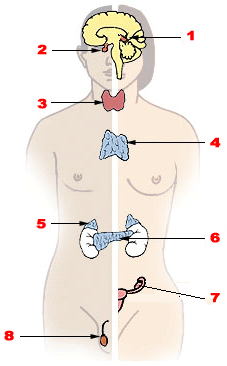
\includegraphics[width=0.2\textwidth]{endokrina.png}
\end{figure}
\vspace{5mm}

\question Varför har vi olika typer av \textbf{muskelvävnad} i kroppen? (\textbf{2 poäng})
\vspace{40mm}

\question Ge exempel på två olika \textbf{signalsubstanser (neurotransmittorer)} och deras funktion. (\textbf{2 poäng})
\vspace{20mm}

\question Vad av följande \textbf{stämmer} om skelettet? (\textbf{2 poäng})
\begin{checkboxes}
    \choice Skelettet skyddar inre organ.
    \choice Alla ben i kroppen är ihåliga.
    \choice Skelettet lagrar mineraler som kalcium och fosfat.
    \choice Röd benmärg bildar blodkroppar.
    \choice Skelettet består bara av död vävnad.
    \choice Leder förbinder olika ben i skelettet.
    \choice Skelettet är viktigt för kroppens rörelse.
    \choice Skelettet producerar hormoner som insulin.
\end{checkboxes}

\break

\vspace{5mm} %5mm vertical space
\begin{center}
\fbox{\fbox{\parbox{6in}{\centering
\textbf{Fördjupande frågor}: svara mer utförligt (\textbf{10 poäng} + 2 bonuspoäng)
}}}
\end{center}

\question
Utifrån bilden beskriv hur en signal överförs mellan två nervceller. Använd relevanta begrepp. (\textbf{3 poäng})
\begin{figure}[h]
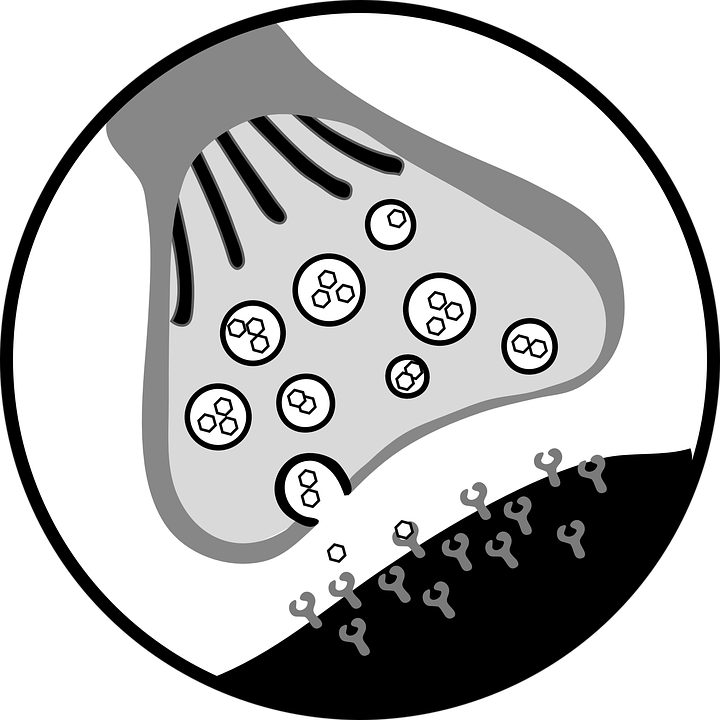
\includegraphics[width=0.4\textwidth]{synaps.png}
\end{figure}
\vspace{30mm}

\question
Organismer har två olika system för kommunikation. Nervsystemet och det endokrina systemet. Vad är för- och nackdelarna med de olika systemen och varför är det viktigt att ha båda två? (\textbf{3 poäng})

\vspace{60mm}

\break

\question Flera däggdjur har både \textbf{endoskolett, exoskelett och hydrostatiskt skelett} (däribland människan). Vad har de olika typerna av skelett för fördelar och varför behövs alla tre? (\textbf{2 poäng})

\vspace{60mm}

\question \textbf{Multipel skleros} (MS) är en autoimmunsjukdom som innebär att det egna immunförsvaret angriper myelinskidorna på nervcellerna. Utifrån dina kunskaper, hur påverkar det nervsystemet och vad skull det kunna få för symptom? (\textbf{2 poäng})

\vspace{80mm}

\question \textbf{BONUS}: Beskriv något du lärt dig och tyckt varit extra intressant, men som inte var med på provet! (\textbf{2 bonuspoäng})

\end{questions}

\end{document}